\chapter{Lecture 14 - Rendering}
\begin{definition}[Rendering]
    \emph{Rendering} is the process of converting input data, such as 3D geometry and material properties, into a final image. To visualize a 3D scene, it must be transformed into a synthetic raster image that can be displayed on a screen.
\end{definition}

To render a scene effectively, an algorithm requires several types of input: \textit{geometric data} (the raw shapes of the objects), \textit{material and texture} (information about how surfaces look and react to light), a \textit{synthetic scene} (the arrangement of these objects in a virtual space), \textit{camera model} (a mathematical description of the "picture-making apparatus").\par
The material categorizes rendering into three families of algorithms:
\begin{itemize}[noitemsep]
    \item \textit{Ray tracing}: tracing the path of light to simulate visual effects
    \item \textit{Path tracing}: a specialized, more advanced form of ray tracing
    \item \textit{Rasterization-based pipeline}: the standard approach for real-time graphics, which converts 3D primitives directly into 2D pixels
\end{itemize}

\subsubsection{The Pinhole camera}
The pinhole camera is a fundamental mathematical model used in computer graphics as a metaphor for the virtual camera, describing the relationship between an observer and a 3D scene.\par
It is modeled as a parallelepiped (a box) where the front face contains an infinitesimally small hole. When the light enters through this hole, the resulting image is formed on the back side of the box, known as the focal plane. \par
This pinhole camera is formed of components: the \textit{viewpoint} is the eye position or the projection center located at the pinhole itself; the \textit{focal distance} (\textit{d}) is the distance between the pinhole (projection center) and the back side of the box where the image forms; while a physical pinhole camera forms an inverted image on the back of the box, computer graphics conventions often assume the existence of an image plane located between the scene and the projection center to simplify calculations.\par
The model allows for precise control over what is visible in the rendered scene. The angle of view \(\theta\) can be controlled by varying the ratio between the focal distance \textit{d} and the height of the image plane \textit{h}.

\begin{figure}[htbp]
    \centering
    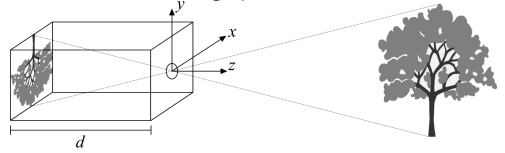
\includegraphics[width=0.5\linewidth]{imgs/lecture14/14.1 pinhole camera.png}
    \caption{Pinhole camera}
    \label{fig:14.1}
\end{figure}

\section{The chain of transformations}
\begin{definition}[chain of transformations]
    The chain of transformations is the technical process of transforming 3D models into 2D synthetic scenes through a sequence of mathematical mappings. 
\end{definition}

\begin{figure}[htbp]
    \centering
    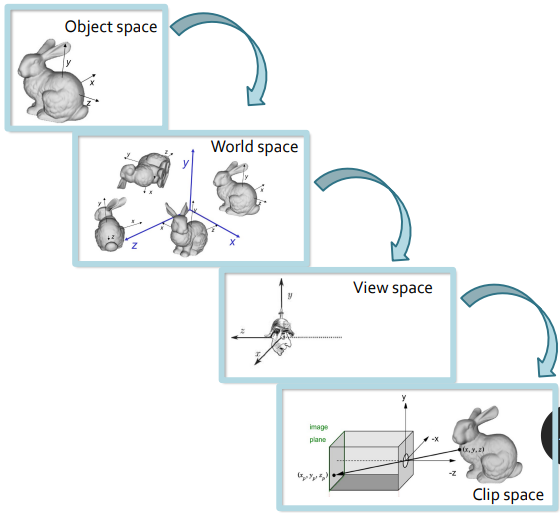
\includegraphics[width=0.4\linewidth]{imgs/lecture14/14.2 chain of transformations.png}
    \caption{The chain of transformations}
    \label{fig:14.2}
\end{figure}

This chain of transformations requires the definition and computation of proper transformations. The hierarchy of space is the following:
\begin{itemize}[noitemsep]
    \item \textbf{Object space} (local space): this is the reference frame where a 3D model is originally defined. Each object has its own space, arbitrarily chosen by the modeler to define its specific point coordinates and normals 
    \item \textbf{World space}: because a scene contains many different models, a common reference system is needed to arrange them; this is the world space. The \textbf{modeling transformation} maps an object from its local space into this shared world space, defining its position, rotation, and scale within the scene
    \item \textbf{View space} (camera/eye space): this space has its origin at the camera center. A second transformation moves objects from the world space into the view space so that their coordinates are relative to where the "eye" sees
    \item \textbf{Clip space}: this is the final destination, aligned with the 2D screen of the output device. Mapping to this space involves projecting 3D elements onto a 2D plane
\end{itemize}

\subsection{Affine transformations}
\begin{definition}[Affine transformations]
    In Euclidean geometry, an affine geometry is a geometric transformation that preserves lines and parallelism.
\end{definition}
We need transformations to translate, scale, rotate, and deform 3D objects, to go from the object to the world space. These transformations are called affine.\par
The affine transformations send points to points, lines to lines, planes to planes, and so on, while \textit { maintaining the ratios of distances} between points on a straight line (midpoint of a segment goes to midpoint of a segment). However, affine transformations do not necessarily preserve angles between lines or distances between points. Examples of affine transformations include translation, rotation, scaling, shear, reflection, and compositions of them in any sequence.

\subsection{Composing transformations}
Often, multiple transformations (like rotating an object and then translating it) need to be combined. The problem is that while rotation and scaling are expressed as products (multiplication), translation is expressed as a sum, making them difficult to combine into a single operation.\par
A possible solution is to use the so-called homogeneous coordinates, that is, a different representation for points and vectors that adds an extra dimension with respect to Cartesian coordinates (a third coordinate w for 2D, or a fourth for 3D).

\subsubsection{Homogeneous coordinates}
Given a 2D point P(x, y) is represented as (\(x_h, y_h, w\)), with \(w \neq 0\). To convert back to original Cartesian coordinates, you divide by the extra dimension: \(x = x_h/w \ and \ y = y_h/w\). By convention, w is usually set to 1 for specific locations (x, y, 1).\par
A big advantage in using this system is that, all affine transformations, including translation, can be represented as \(3 \times 3 \) matrices (for 2D) or \(4 \times 4\) matrices (for 3D). This facilitates the mathematical concatenation of several transformations into one by simply multiplying the matrices. This results in a single "master matrix" that can be applied to every point in a 3D model in one step. \par
We can also use homogeneous coordinates to remove points/vectors ambiguity, by setting w coordinates to 1, we have points (locations); and when w = 1, we have vectors (directions) representing "points at infinity".

\section{Ray tracing}
\begin{definition}
    Ray tracing is a rendering paradigm that simulates the way light behaves in the real world by following its path.
\end{definition}
The main idea of the ray tracing is tracing backwards. In nature, light rays travel from a source, bounce off objects, and eventually enters our eyes. Because the vast majority of light rays in a scene never reach the observer, simulating all of them would be a vast amount of energy. So, instead of tracing light from the source, ray tracing works backward. For each pixel on the screen, the algorithm shoots a ray, called a \textbf{primary ray}, from the viewpoint into the scene. And the algorithm finds where that ray intersects with the closest primitive (object) in the 3D scene. The color of that pixel is then determined by the properties of the object hit at that specific point. \par

\subsubsection{Secondary rays}
One of the primary advantages of ray tracing is that it handles complex optical phenomena "naturally" through the use of secondary rays:
\begin{itemize}[noitemsep]
    \item To see if a point is in shadow, the algorithm shoots a "\textbf{shadowing ray}" from the intersection point toward the light source. If it hits an object on the way, the point is in shadow.
    \item If the ray hits a mirror-like surface, a new "\textbf{reflection ray}" is bounced off the surface to see what other objects are reflected in it.
    \item For semi-transparent objects like glass or water, the algorithm calculates a "\textbf{refracted ray}" that passes through the material, allowing for a realistic simulation of transparency.
\end{itemize}

\begin{figure}[htbp]
    \centering
    
    \begin{subfigure}[b]{0.45\textwidth}
        \centering
        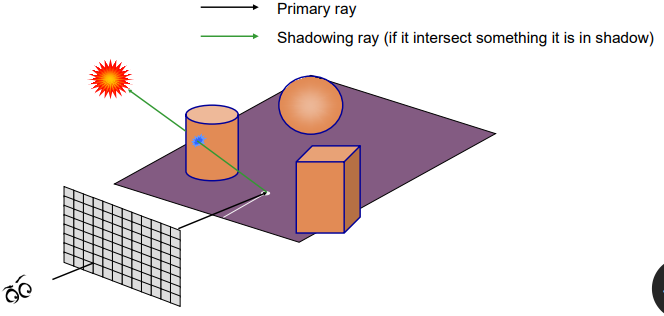
\includegraphics[width=0.8\linewidth]{imgs/lecture14/14.3 ray tracing and shadow ray.png}
        \caption{Shadowing ray}
        \label{fig:14.3a}
    \end{subfigure}
    \hfill
    \begin{subfigure}[b]{0.45\textwidth}
        \centering
        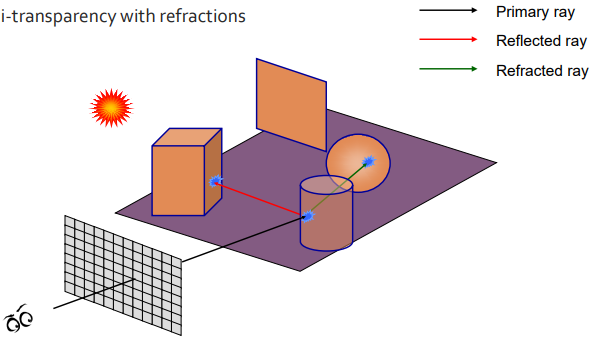
\includegraphics[width=0.8\linewidth]{imgs/lecture14/14.4 ray tracing and reflectio refraction ray.png}
        \caption{Reflection and refraction rays}
        \label{fig:14.3b}
    \end{subfigure}

    \caption{Ray tracing: primary and secondary rays}
    \label{fig:14.3}
\end{figure}

\subsubsection{Primitives and geometry}
Ray tracing offers more freedom in the types of shades it can render compared to other methods. While most real-time systems rely on triangles, ray tracing can intersect rays with any mathematical primitive that has a defined intersection formula, including spheres, implicit surfaces, and Geometric Solid Modeling (GSM).

\subsubsection{Computational cost}
Historically, ray tracing was considered "too slow" for real-time use because the core operation, computing the intersection between a 3D ray and 3D primitives, is complex. However, the cost is actually sublinear relative to the number of objects in the scene, provided the right data structures are used. And to speed up calculations, spatial indexing is used, a specialized hierarchical or hashing-based data structures that allow the algorithm to quickly skip parts of the scene the ray won't hit.\par
Modern GPUs, like NVIDIA RTX, now combine ray tracing with traditional methods to achieve the effects in real-time.

\section{Rasterization}
Rasterization is the alternative to ray tracing, which is the standard method for real-time graphics. While ray tracing works by shooting rays from the observer for each pixel, rasterization takes the opposite approach: \textbf{it takes each 3D object and determines which pixels it covers on the screen}.
\begin{definition}[Rasterization]
    Rasterization is a rendering paradigm that converts 3D geometric data into a 2D raster image by determining which pixels on the screen are covered by each 3D object.
\end{definition}

Because modern GPUs are highly optimized for rasterization, almost every 3D scene is decomposed entirely into triangles before being rendered. Rasterization is also frequently called the \textbf{T \& L pipeline}, consisting of two primary computational goals:
\begin{itemize}[noitemsep]
    \item \textbf{Transform}: the algorithm projects 3D primitives (geometric shapes) from their world coordinates into the 2D "screen space" of the output device
    \item \textbf{Lighting}: the algorithm computes the final color for every part of the scene, taking into account the geometry, the light sources, and the optical characteristics of the material
\end{itemize}

\subsubsection{Rasterization process}
The process flows through four distinct stages to turn a vertex into a pixel:
\begin{enumerate}[noitemsep]
    \item Per-vertex transformations: individual vertices and their attributes are moved into the correct coordinate spaces
    \item Primitive processing: the vertices are assembled into basic shapes, while points and lines are possible, triangles are the universal standard because graphics HW is specifically optimized to process them
    \item Rasterization: the core step where a 2D shape on the screen is filled with a grid of fragments. A fragment is essentially a "potential pixel" that carries all the data necessary to compute a final color.
    \item Per-fragment computation: the final color of each fragment is determined, often by accessing texture RAM to apply images to the surface, before the results are written to the frame buffer.
\end{enumerate}

\subsubsection{Attributes Interpolation and Perspective correction}
During rasterization, the values defined at the corners of the triangle, the vertices, must be spread across the entire surface. If  \textit{Barycentric coordinates} are used, the algorithm performs a linear interpolation of attributes like colors or normals across the face of a triangle. If \textit{Perspective correction} is used, a simple linear interpolation of texture coordinates across a triangle can cause visual distortion due to the way perspective works. Rasterization HW must apply a perspective correction formula using the depth (w) coordinate to ensure textures appear correctly aligned as they recede into the distance.

\begin{figure}
    \centering
    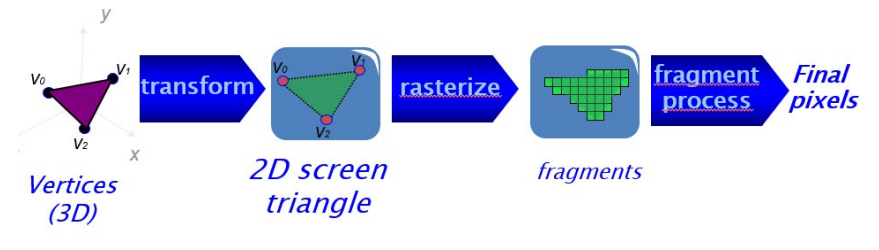
\includegraphics[width=0.5\linewidth]{imgs/lecture14/14.5 rasterization pipeline.png}
    \caption{Rasterization-based rendering}
    \label{fig:14.4}
\end{figure}
\subsubsection{Advantages and limitation}
Rasterization remains the dominant paradigm despite the rise of ray tracing, thanks to the ease of \textbf{parallelism}, making it perfectly suited for the architecture of modern GPUs; the high \textbf{scalability} of image resolution, meaning increasing the number of pixels on a screen has a more predictable performance cost than in ray tracing. \par
However, a historical disadvantage of rasterization is that it cannot naturally handle "global" effects like shadows or reflections. But designers have developed "clever" advanced algorithms to approximate these effects with compromise-level quality in real-time.

\section{Ray tracing Vs Rasterization}
The debate between ray tracing and rasterization stems from their fundamentally different approaches to generating an image from 3D data. It is a choice between processing the scene "pixel by pixel" Vs "primitive by primitive".\par
Quick recap, in ray tracing, for each pixel on the screen, the algorithm checks every geometric primitive in the screen to see if it is hit by a ray; in rasterization, for each geometric primitive (usually a triangle), the algorithm determines which pixels on the screen it covers.

\subsubsection{Advantages of \textit{Ray tracing}}
Ray tracing is often preferred for high-fidelity, "off-line" rendering, such as in movies by Pixar or DreamWorks, for several reasons:
\begin{itemize}[noitemsep]
    \item \textbf{Global effects} --> it naturally handles complex optical phenomena like shadows, specular reflections, and refractions
    \item \textbf{Conceptual simplicity }--> the underlying algorithm is straightforward, you simply trace the path of light
    \item \textbf{Primitive freedom} --> it is easier to calculate the intersection of a ray with complex mathematical shapes (spheres, implicit surfaces) than it is to project and fill those shapes as pixels
    \item \textbf{Scene scalability} --> if a specialized data structure for "spatial indexing" is used, the computational cost can be sublinear relative to the number of objects in the scene
\end{itemize}

\subsubsection{Advantages of \textit{Rasterization}}
Rasterization is the standard for "real-time" rendering, such as video games and web previews, because of its efficiency:
\begin{itemize}[noitemsep]
    \item \textbf{Parallelism and HW optimization} --> the algorithm is easily parallelizable and was the first to receive specialized HW support, GPUs
    \item \textbf{Resolution scalability} --> it scaled better with image resolution (the number of pixels) than ray tracing
    \item \textbf{Handling dynamic data} --> it is generally easier to manage scenes where objects are constantly moving
    \item \textbf{Speed} --> it is inherently fast because it only processes the specific pixels covered by a primitive rather than checking every primitive for every pixel
\end{itemize}

\subsubsection{The reality of the debate...}
The traditional boundaries between these two methods are blurring. The current state is that \textit{rasterization is fast, but needs cleverness to support complex visual effects; ray tracing supports complex visual effects, but needs cleverness to be fast}.\par
A clever rasterization utilizes real-time engines that use algorithms and approximations to simulate the reflections and shadows that ray tracing produces naturally. While clever ray tracing uses efficient spatial queries to avoid being slow. \par
Modern technology, such as NVIDIA RTX, has effectively ended the binary debate by combining both rasterization and ray tracing within the same HW to achieve high-quality visual effects at real-time speeds.